\title{[Lab3] Diabetic Retinopathy Detection}
\author{0616014 楊政道}
\maketitle
\thispagestyle{fancy}
\section{Introduction}
\subsection{Lab Objective}
\paragraph{}
In this assignment, I will use pytorch to construct ResNet to analysis diabetic retinopathy. Finally, plot the confusion matrix and accuracy plot during trainging and testing.
\subsection{Dataset}
\paragraph{}
There are 28099 images as training dataset and 7025 images as testing dataset. The image size is 512 by 512.
\begin{figure}[!ht]
    \begin{center} 
        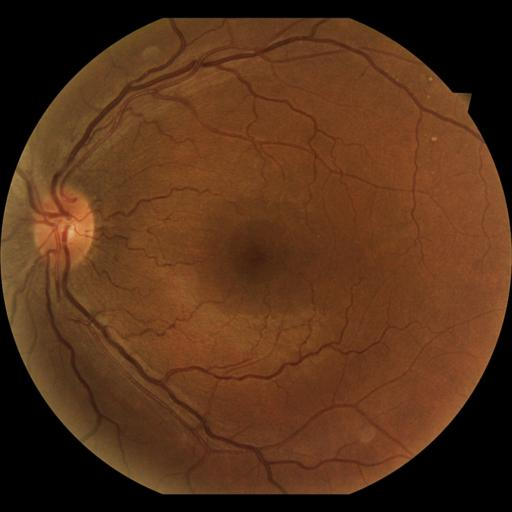
\includegraphics[width=5cm]{dataset_example.jpeg}
        \caption{Dataset Sample Image}
    \end{center} 
\end{figure}
\subsection{Project Structure}
\dirtree{%
.1 DLP\_LAB3\_0616014\_楊政道.zip.
.2 data/.
.3 dataloader.py.
.2 models.py
.2 weight/.
.3 record.json.
.2 train.py.
.2 evaluate.py.
}
\subsubsection{data/dataloader.py}
\paragraph{}
To generate the pytorch dataloader for our training and testing data.
\subsubsection{models.py}
\paragraph{}
To define the structure of ResNet and some api for ResNet18 and ResNet50.
\subsubsection{weight/record.json}
\paragraph{}
To mentain the maximum test accuracy. If we have higher test accuracy, we will replace the weight and update the record file. The model parameters will be stored in weight directory.
\subsubsection{train.py}
\paragraph{}
To define the Trainer class and train networks.
\subsubsection{evaluate.py}
\paragraph{}
It will load the network parameters we have stored and evaluate the network.
\section{Experiment Setup}
\subsection{The details of ResNet model}
\subsubsection{ResNet}
\paragraph{}
I use pytorch api to construct the ResNet architecture. The only different part is the last layer of the model, we use a new fully-connected layer as the classification layer.
\paragraph{}
The reason why the residual shortcut can avoid vanishing gradient problems is that the gradient of the weight at least 1, so there are still gradient to be propagated back to the previous layer. 
\begin{lstlisting}[language=Python]
class ResNet(nn.Module):
    def __init__(self, num, pretrained=False, lr=1e-4):
        super(ResNet, self).__init__()

        self.pretrained = pretrained
        self.num = num
        pretrained_model = torchvision.models.__dict__['resnet{}'.format(num)](pretrained=pretrained)
        self.conv1 = pretrained_model._modules['conv1']
        self.bn1 = pretrained_model._modules['bn1']
        self.relu = pretrained_model._modules['relu']
        self.maxpool = pretrained_model._modules['maxpool']
        self.layer1 = pretrained_model._modules['layer1']
        self.layer2 = pretrained_model._modules['layer2']
        self.layer3 = pretrained_model._modules['layer3']
        self.layer4 = pretrained_model._modules['layer4']
        self.avgpool = nn.AdaptiveAvgPool2d(1)
        self.classify = nn.Linear(pretrained_model._modules['fc'].in_features, 5)

        del pretrained_model
\end{lstlisting}
\subsubsection{ResNet18}
\begin{lstlisting}[language=Python]
def ResNet18(device, pretrained=False):
    return ResNet(18, pretrained).to(device)
\end{lstlisting}
\subsubsection{ResNet50}
\begin{lstlisting}[language=Python]
def ResNet50(device, pretrained=False):
    return ResNet(50, pretrained).to(device)
\end{lstlisting}
\subsection{The details of Dataloader}
\paragraph{}
There are two main function need to be implemented, \_\_len\_\_ and \_\_getitem\_\_. The details of \_\_len\_\_ function are returning the length of the dataset simply. The details of \_\_getitem\_\_ are loading the image data according to the given index and doing some transformations(RandomHorizontalFlip, ToTensor, normalize).
\begin{lstlisting}[language=Python]
class RetinopathyLoader(data.Dataset):
    def __init__(self, root, mode, arg=None):
        self.root = root
        self.img_name, self.label = getData(root, mode)
        self.mode = mode
        trans=[]
        if arg:
            trans += arg
        self.transforms = transforms.Compose(trans)

    def __len__(self):
        return len(self.img_name)

    def __getitem__(self, index):
        img = PIL.Image.open(self.root + 'jpeg/' + self.img_name[index] + '.jpeg')
        img = self.transforms(img)
        label = self.label[index]
        return img, label
\end{lstlisting}
\subsection{Evaluation through the confusion matrix}
\begin{figure}[!ht]
    \begin{center} 
        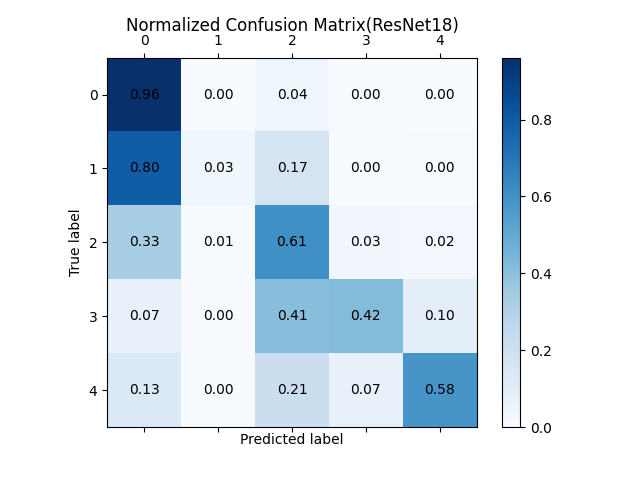
\includegraphics[width=10cm]{Conf-ResNet18.png}
        \caption{Confusion Matrix in ResNet18}
    \end{center} 
\end{figure}
\begin{figure}[!ht]
    \begin{center} 
        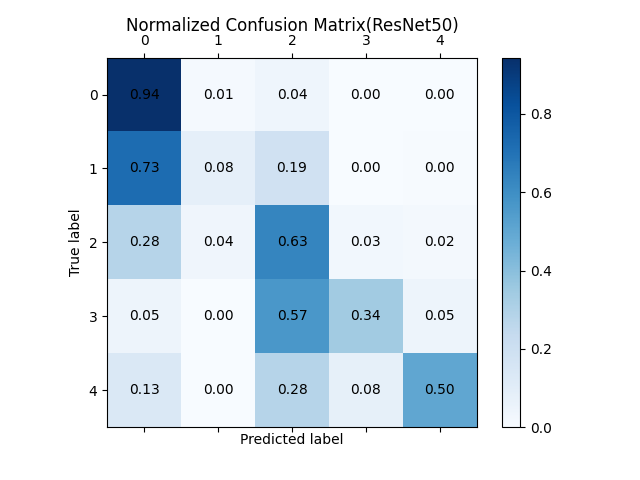
\includegraphics[width=10cm]{Conf-ResNet50.png}
        \caption{Confusion matrix in ResNet50}
    \end{center} 
\end{figure}
\section{Experimental Result}
\subsection{Highest Test Accuracy}
\begin{center}
\begin{tabular}{ |c|c|  }
\hline
Model & Max Test Acc\\
\hline
ResNet18\_pretrained & 82.16\% \\
ResNet18 & 73.35\% \\
ResNet50\_pretrained & 81.34\% \\
ResNet50 & 75.00\% \\
\hline
\end{tabular}
\end{center}
\paragraph{}
First, I train pretrained ResNet18 with 10 epochs and pretrained ResNet50 with 5 epochs and store the weights which performs best at test dataset.
\paragraph{}
Then, I decrease the initial learning rate and train from the weight I store at the previous stage.
\subsection{Comparison figures}
\subsubsection{ResNet18}
\begin{figure}[!ht]
    \begin{center} 
        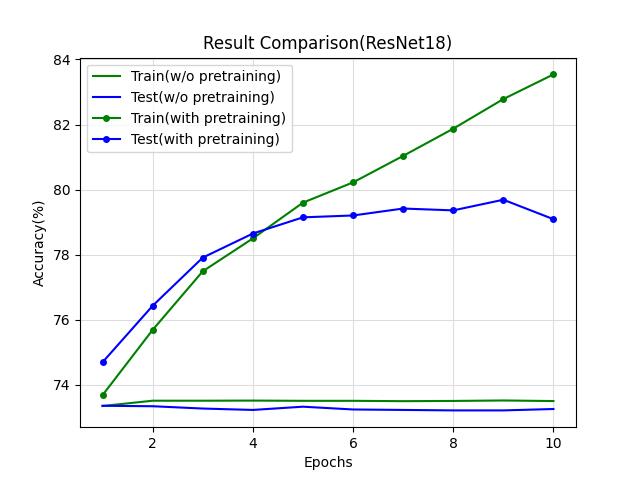
\includegraphics[width=8cm]{Result-ResNet18.png}
        \caption{Result comparison(ResNet18)}
    \end{center} 
\end{figure}
\subsubsection{ResNet50}
\begin{figure}[!ht]
    \begin{center} 
        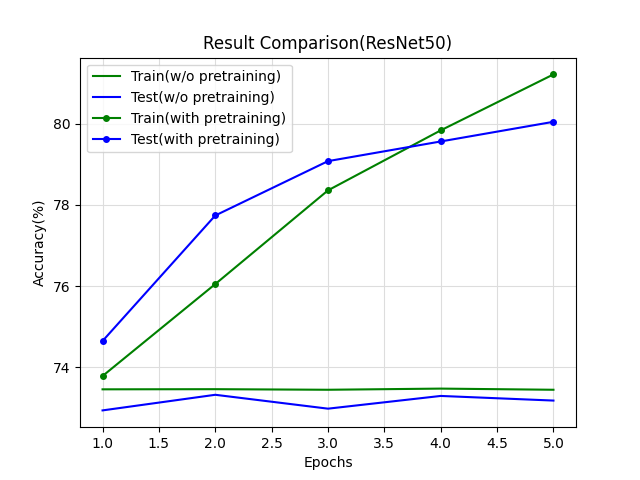
\includegraphics[width=8cm]{Result-ResNet50.png}
        \caption{Result comparison(ResNet50)}
    \end{center} 
\end{figure}
\section{Discussion}
\subsection{Data augmentation}
\subsubsection{RandomHorizontalFlip}
\paragraph{}
Because there are left-eye and right-eye images in this dataset, I can use random horizontal flip to strong the dataset.
\subsubsection{Normalize}
\paragraph{}
In order to use pretrain weight, I need to make the input value into correct range. According the code on the pytorch github, the input need to be scale into [0, 1] by ToTensor transformation and use normalize transformation(mean=[0.485, 0.456, 0.406], std=[0.229, 0.224, 0.225])
\subsubsection{Some observations on prediction}
\begin{figure}[!ht]
    \begin{center} 
        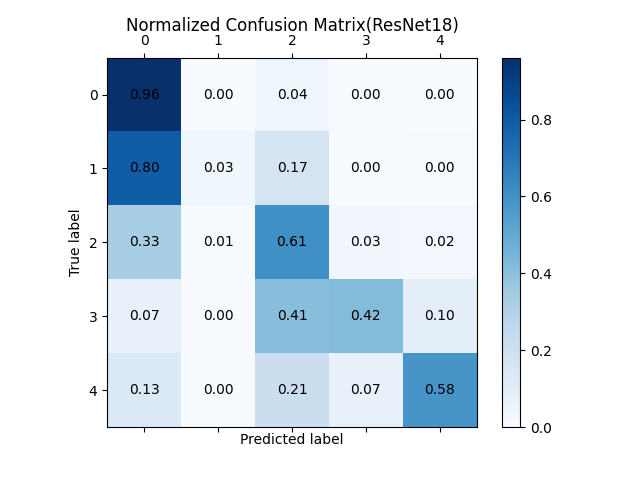
\includegraphics[width=10cm]{Conf-ResNet18.png}
        \caption{Confusion Matrix in ResNet18}
    \end{center} 
\end{figure}
\paragraph{}
My model predicts many class1 to class0. There are some reasons.
\begin{itemize}
    \item The number of the images in class0 is more than class1 significantly.
    \item There are no obvious features to seperate class0 and class1.
\end{itemize}
